\documentclass[11pt,a4paper]{article}
\usepackage[utf8]{inputenc}
\usepackage[T1]{fontenc}
\usepackage[spanish,provide=*]{babel}
\addto\captionsspanish{\renewcommand{\tablename}{Tabla}}
\usepackage{lmodern}
\usepackage{microtype}
\usepackage[margin=2.5cm]{geometry}
\usepackage{amsmath,amssymb}
\usepackage{graphicx}
\usepackage{booktabs}
\usepackage{adjustbox}
\usepackage{pdflscape}
\usepackage{float}
\usepackage[font=small,labelfont=bf]{caption}
\usepackage{enumitem}
\usepackage{xcolor}
\usepackage{listings}
\usepackage[round]{natbib}
\usepackage[hidelinks]{hyperref}
\setlength{\parskip}{0.5em}
\setlength{\parindent}{0pt}
\setlist{itemsep=0.2em}

% Texto en rojo = algo que hay que revisar/actualizar después de volver a correr el do-file.
% Para sacar el color: \renewcommand{\revisar}[1]{#1}
\newcommand{\revisar}[1]{\textcolor{red}{#1}}
% Inserta una tabla exportada desde Stata (se achica si no entra)
\newcommand{\tabla}[1]{\begin{adjustbox}{max width=\linewidth, max totalheight=0.72\textheight}\input{#1}\end{adjustbox}}
% Figura que todavía no existe (se genera al correr el do-file): muestra un recuadro
\newcommand{\figura}[2][0.75\linewidth]{\IfFileExists{#2}{\includegraphics[width=#1]{#2}}{\fbox{\parbox{\dimexpr#1-2\fboxsep-2\fboxrule\relax}{\centering\vspace{2em}\textcolor{red}{Figura pendiente: se genera al correr el do-file}\\[0.5em]\texttt{\detokenize{#2}}\vspace{2em}}}}}
% Notas al pie de tablas
\newcommand{\notas}[1]{\par\vspace{0.3em}\begin{minipage}{0.92\linewidth}\footnotesize\textit{Notas:} #1\end{minipage}}
% Consignas en cursiva
\newcommand{\consigna}[1]{\par\textit{#1}\par}

\lstset{
  language={},
  basicstyle=\ttfamily\scriptsize,
  breaklines=true,
  columns=fullflexible,
  keepspaces=true,
  showstringspaces=false,
  frame=single,
  rulecolor=\color{gray!50},
  commentstyle=\color{gray},
  morecomment=[l]{*\ },
  morecomment=[l]{//},
  morecomment=[s]{/*}{*/},
  tabsize=4,
  inputencoding=utf8,
  extendedchars=true,
  literate={á}{{\'a}}1 {é}{{\'e}}1 {í}{{\'i}}1 {ó}{{\'o}}1 {ú}{{\'u}}1
           {Á}{{\'A}}1 {É}{{\'E}}1 {Í}{{\'I}}1 {Ó}{{\'O}}1 {Ú}{{\'U}}1
           {ñ}{{\~n}}1 {Ñ}{{\~N}}1 {ü}{{\"u}}1 {Ü}{{\"U}}1
           {¿}{{?`}}1 {¡}{{!`}}1 {’}{{'}}1 {‘}{{`}}1 {“}{{``}}1 {”}{{''}}1
           {ã}{{\~a}}1 {õ}{{\~o}}1 {â}{{\^a}}1 {ê}{{\^e}}1 {ô}{{\^o}}1 {à}{{\`a}}1
           {Ã}{{\~A}}1 {Õ}{{\~O}}1 {Â}{{\^A}}1 {Ê}{{\^E}}1 {Ô}{{\^O}}1 {Ç}{{\c C}}1 {×}{{$\times$}}1
           {°}{{$^\circ$}}1 {–}{{--}}1 {—}{{---}}1 {·}{{$\cdot$}}1 {ç}{{\c c}}1
}
\begin{document}

\begin{center}
{\Large\bfseries Problem Set 6: Diferencias en diferencias}\\[0.5em]
E178: Economía Aplicada --- Universidad de San Andrés\\
Fecha de entrega: 28 de octubre de 2024\\[0.5em]
\textbf{Integrantes:} Juan Batalla, Nina Di Costanzo Pereira, Catalina Gallardo e Ignacio Yenarópulos
\end{center}

Este problem set se basa en \citet{cheng}, que explotan la adopción escalonada de la \textit{Castle Doctrine} (que amplió el derecho a usar fuerza letal en defensa propia) en 21 estados de EE.UU. entre 2005 y 2009 para evaluar su efecto sobre el crimen. Usamos la base \texttt{castle.dta}, un panel de los 50 estados entre 2000 y 2010.

\section*{1. Replicación de la Tabla 4}

Estimamos modelos de efectos fijos de estado y año (diferencias en diferencias con adopción escalonada):
\[
\ln(\text{Crimen}_{it})=\beta\,\text{CDL}_{it}+\alpha_i+\gamma_t+X_{it}'\delta+\varepsilon_{it},
\]
donde $\text{CDL}_{it}$ es la proporción del año $t$ en la que la ley estuvo vigente en el estado $i$ (vale 1 en los años posteriores a la adopción y una fracción en el año de adopción). Las columnas agregan sucesivamente efectos fijos región-año, controles que varían en el tiempo, una variable para los dos años previos a la adopción (test de falsificación), tasas contemporáneas de hurto y robo de vehículos, y tendencias lineales por estado. La consigna indica ignorar los pesos poblacionales; para poder comparar con el paper presentamos ambas versiones: las columnas 1--6 están ponderadas por población y las columnas 7--12 son las estimaciones sin ponderar. Los errores estándar están clusterizados por estado.

\begin{landscape}
\begin{table}[H]\centering
\caption{Efectos disuasivos de la Castle Doctrine: burglary, robbery y aggravated assault}\label{tab:t4}
\scriptsize
\begin{adjustbox}{max width=\linewidth, max totalheight=0.78\textheight}
\begin{tabular}{c}
\textbf{Panel A: log(tasa de burglary)}\\
\input{"../output/Tabla 4a.tex"}\\[0.5em]
\textbf{Panel B: log(tasa de robbery)}\\
\input{"../output/Tabla 4b.tex"}\\[0.5em]
\textbf{Panel C: log(tasa de aggravated assault)}\\
\input{"../output/Tabla 4c.tex"}
\end{tabular}
\end{adjustbox}
\notas{Cada columna de cada panel es una regresión distinta; la unidad de observación es estado-año. Columnas 1--6: MCO ponderado por población; columnas 7--12: sin ponderar. Errores estándar clusterizados por estado entre paréntesis. Los controles incluyen tasas de policía y de encarcelamiento, gasto en asistencia social, ingreso mediano, tasa de pobreza, desempleo y demografía. Los delitos contemporáneos son las tasas (en logaritmos) de hurto y robo de vehículos. * $p<0.10$, ** $p<0.05$, *** $p<0.01$.}
\end{table}
\end{landscape}

Con la ley medida como la proporción del año en vigencia y los delitos contemporáneos definidos como en el paper, replicamos la Tabla 4 de \citet{cheng} prácticamente sin diferencias (Tabla~\ref{tab:t4}). Cada coeficiente se interpreta como el cambio porcentual aproximado en la tasa de delito cuando la ley está vigente todo el año. Los resultados no muestran efectos disuasivos: si la ley disuadiera a los delincuentes, esperaríamos coeficientes negativos, pero ninguno lo es. En burglary, el coeficiente de la especificación más simple ponderada es positivo y significativo (0.078), pero cae a 0.029 y deja de ser significativo al agregar efectos fijos región-año, lo que indica que reflejaba shocks regionales. En robbery los coeficientes son positivos y pequeños (entre 0.02 y 0.05) y solo son significativos en algunas especificaciones (con delitos contemporáneos o tendencias por estado). En aggravated assault ningún coeficiente es significativo. El coeficiente de los dos años previos a la adopción es chico y no significativo en los tres paneles, lo que no sugiere que los delitos ya estuvieran cambiando antes de la ley en los estados que la adoptaron. La conclusión, igual que en el paper, es que la Castle Doctrine no redujo estos delitos.

\section*{2. Estimador de Callaway y Sant'Anna}

Cuando la adopción es escalonada y los efectos son heterogéneos entre grupos o en el tiempo, el estimador de efectos fijos en dos sentidos (TWFE) puede estar sesgado, porque usa a los estados ya tratados como controles de los que se tratan después (comparaciones ``prohibidas'' que pueden recibir ponderaciones negativas). \citet{cs} estiman por separado el efecto para cada grupo $g$ (estados que adoptan la ley en el año $g$) y cada año $t$, $ATT(g,t)$, comparando la evolución del outcome del grupo entre $g-1$ y $t$ con la de los estados nunca tratados o todavía no tratados en $t$. Luego agregan esos efectos. Replicamos la columna 1 del panel C (sin controles, ponderada por población), usando como grupo de comparación a los estados nunca tratados y a los aún no tratados.

\begin{table}[H]\centering
\caption{Estimador de Callaway y Sant'Anna: ATT simple y estudio de eventos}\label{tab:cs}
\scriptsize
\tabla{"../output/Callaway_SantAnna.tex"}
\notas{Variable dependiente: log(tasa de aggravated assault). Ponderado por población; grupo de comparación: estados nunca tratados y aún no tratados. Tm$k$ (Tp$k$): $k$ años antes (después) de la adopción. Los ATT pre-tratamiento usan como base el año anterior. Pre\_avg y Post\_avg: promedio de los efectos antes y después de la adopción. Errores estándar entre paréntesis. * $p<0.10$, ** $p<0.05$, *** $p<0.01$.}
\end{table}

El ATT simple es de 0.027, con un error estándar de 0.023: en promedio, en los años posteriores a la adopción, la tasa de aggravated assault de los estados tratados fue alrededor de 2.7\% mayor que la que habrían tenido sin la ley, pero el efecto no es significativo. Es menor que el estimado por TWFE (0.043) y, como este, no indica una reducción de los delitos. Los efectos por grupo (Figura~\ref{fig:groups}) son positivos pero imprecisos para los grupos 2006 (13 estados), 2007 (4 estados) y 2008 (2 estados). El grupo 2009 tiene un solo estado (Montana), y sus estimaciones oscilan mucho de un año a otro.

\begin{figure}[H]\centering
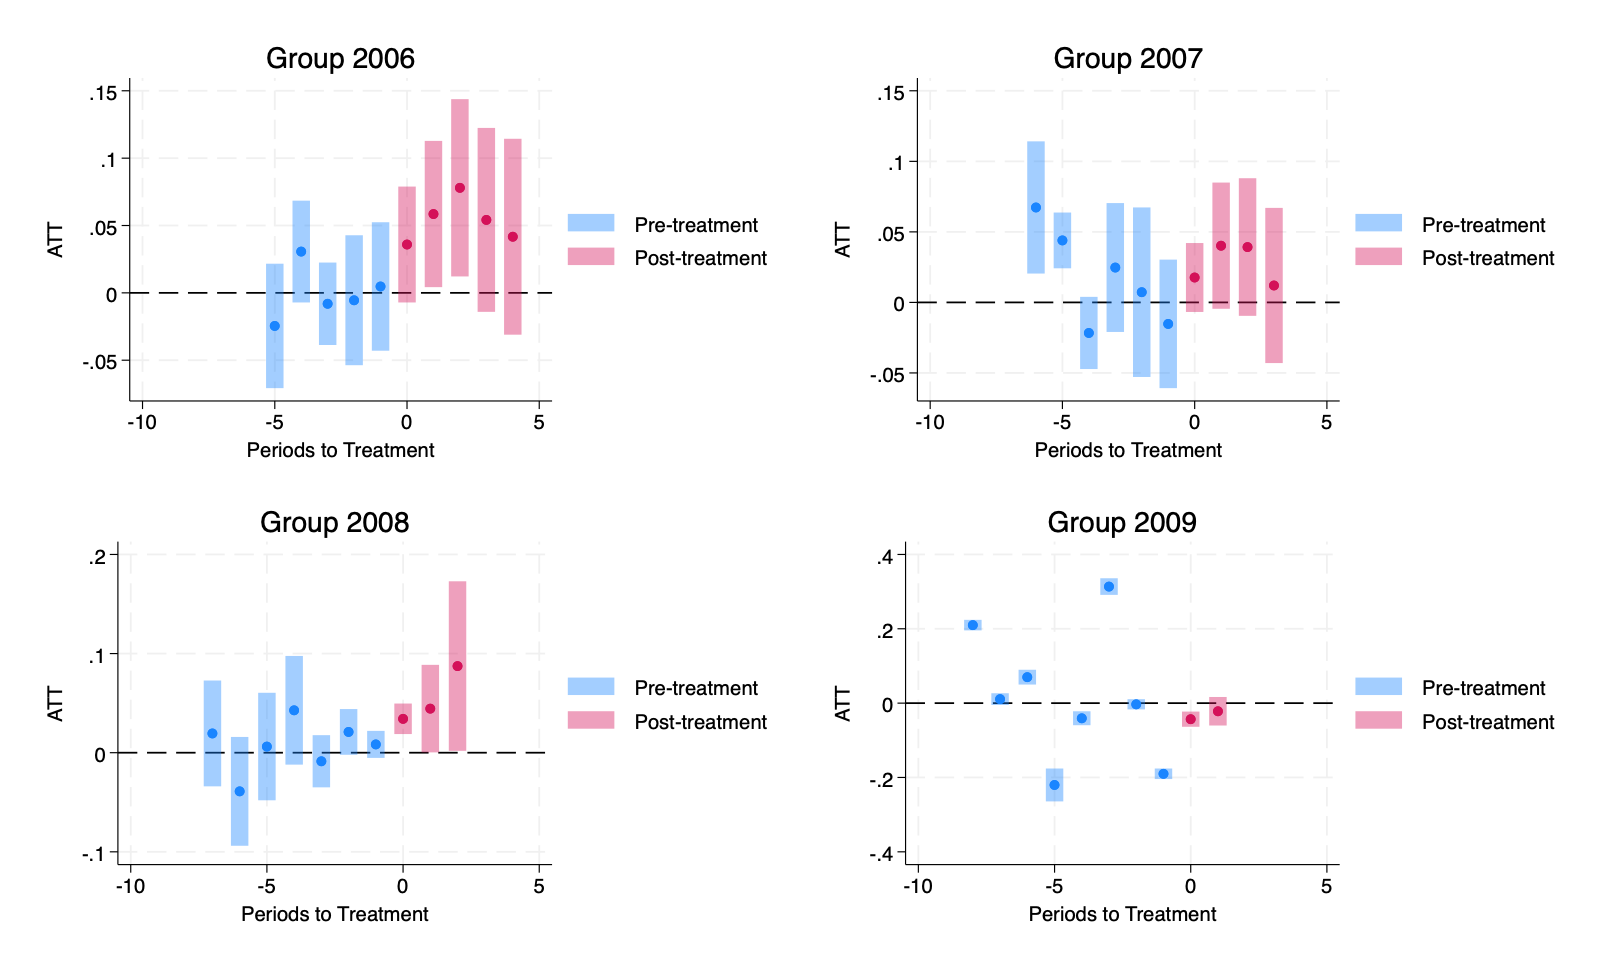
\includegraphics[width=0.85\linewidth]{../output/Grafico.png}
\caption{$ATT(g,t)$ para los grupos 2006, 2007, 2008 y 2009.}\label{fig:groups}
\end{figure}

\begin{figure}[H]\centering
\figura[0.7\linewidth]{../output/Event_study_CS.png}
\caption{Estudio de eventos (Callaway y Sant'Anna)}\label{fig:evcs}
\end{figure}

La Figura~\ref{fig:evcs} muestra el estudio de eventos, que agrega los efectos según los años desde la adopción. En los siete años previos a la adopción los coeficientes son chicos (entre $-0.001$ y $0.039$) y, salvo uno significativo al 10\%, no son significativos, lo que es consistente con tendencias paralelas. La excepción es ocho años antes de la adopción ($0.21$), un coeficiente que se estima solo con Montana. Después de la adopción los efectos son positivos y chicos (entre 0.010 y 0.054, significativos al 5\% en los tres primeros años) y negativos cinco años después ($-0.166$), cuando solo queda Florida en la muestra.

El test conjunto de que todos los $ATT(g,t)$ pre-tratamiento son cero rechaza con fuerza ($\chi^2(30)=37{,}397$, p-valor $<0.001$). Sin embargo, el resultado está dominado por las celdas de grupos con un solo estado, sobre todo Montana (grupo 2009), cuyos $ATT(g,t)$ previos son grandes (de hasta $\pm0.3$) y tienen errores estándar artificialmente chicos: con un único estado tratado, la varianza del efecto no se puede estimar bien. Si miramos el estudio de eventos agregado, los coeficientes de los cinco años previos son prácticamente cero. Por eso no interpretamos el rechazo como evidencia clara contra las tendencias paralelas, aunque sí como una advertencia sobre los grupos chicos. En cualquier caso, ningún test ``valida'' el supuesto: el supuesto se refiere a lo que habría pasado después de la adopción sin la ley, algo que no se observa, y el test solo evalúa si las tendencias previas eran paralelas.

\section*{3. Imputation estimator de Borusyak, Jaravel y Spiess}

El estimador de imputación \citep{bjs} estima un modelo con efectos fijos de estado y de año usando \emph{solo} las observaciones no tratadas (los estados nunca tratados y los años previos a la adopción de los tratados). Con esos efectos fijos imputa el resultado contrafáctico sin tratamiento, $\hat Y_{it}(0)=\hat\alpha_i+\hat\gamma_t$, para cada observación tratada, y el efecto es el promedio de $Y_{it}-\hat Y_{it}(0)$. A diferencia de TWFE, nunca usa a los estados ya tratados como controles. Estimamos la columna 1 del panel C sin controles, ponderando por población.

\begin{table}[H]\centering
\caption{Imputation estimator: efecto promedio, efectos por horizonte y pre-tendencias}\label{tab:bjs}
\scriptsize
\tabla{"../output/Imputation.tex"}
\notas{Variable dependiente: log(tasa de aggravated assault). Ponderado por población. tau$h$: efecto $h$ años después de la adopción. pre$k$: coeficiente $k$ años antes de la adopción, estimado en las observaciones no tratadas. Errores estándar entre paréntesis. * $p<0.10$, ** $p<0.05$, *** $p<0.01$.}
\end{table}

\begin{figure}[H]\centering
\figura[0.7\linewidth]{../output/Event_study_BJS.png}
\caption{Estudio de eventos (imputation estimator)}\label{fig:evbjs}
\end{figure}

El efecto promedio estimado es 0.038, con un error estándar de 0.033, así que no es significativo. Es muy similar al de TWFE (0.043) y algo mayor que el de Callaway y Sant'Anna (0.027). Por horizonte, los efectos son positivos y chicos durante los primeros cuatro años (entre 0.017 y 0.068, significativos solo al 10\% uno y dos años después de la adopción) y negativos cinco años después ($-0.162$), cuando nuevamente solo se observa a Florida. Los coeficientes de pre-tendencias son positivos y de magnitud similar entre sí (0.045 para uno, dos y tres años antes; 0.038 y 0.022 para cuatro y cinco años antes), pero solo uno es significativo al 10\% y el test conjunto no rechaza la hipótesis de que todos son cero ($F=1.10$, p-valor $=0.375$). Es decir, con este estimador no hay evidencia estadística de tendencias previas, aunque el patrón de coeficientes positivos sugiere tomar el supuesto con cierta cautela.

Los tres estimadores coinciden en lo importante: el efecto de la Castle Doctrine sobre los aggravated assaults es positivo, chico y no significativo, así que no hay evidencia de efectos disuasivos. Las diferencias en las magnitudes vienen de cómo cada método construye el contrafáctico. TWFE promedia comparaciones que incluyen a estados ya tratados como controles. Callaway y Sant'Anna comparan cada grupo con los no tratados usando solo el año previo a la adopción como base. El estimador de imputación usa todos los períodos no tratados para estimar los efectos fijos, lo que lo hace más eficiente si las tendencias paralelas valen en todos los períodos, pero más sensible a violaciones en los años más alejados de la adopción.

\begin{thebibliography}{9}
\bibitem[Borusyak et al.(2024)]{bjs} Borusyak, K., Jaravel, X., y Spiess, J. (2024). Revisiting event-study designs: robust and efficient estimation. \textit{Review of Economic Studies}, 91(6), 3253--3285.
\bibitem[Callaway y Sant'Anna(2021)]{cs} Callaway, B., y Sant'Anna, P. H. C. (2021). Difference-in-differences with multiple time periods. \textit{Journal of Econometrics}, 225(2), 200--230.
\bibitem[Cheng y Hoekstra(2013)]{cheng} Cheng, C., y Hoekstra, M. (2013). Does strengthening self-defense law deter crime or escalate violence? Evidence from expansions to castle doctrine. \textit{Journal of Human Resources}, 48(3), 821--854.
\end{thebibliography}

\newpage
\appendix
\section*{Apéndice: código}
\lstinputlisting{../programs/ps6.do}

\end{document}
